%\graphicspath{{/home/arbon/Pictures/Screenshots/}} % path to graphics
\graphicspath{{~/Documents/SftAppDvTech/FirstTask/TheBasics}}
\chapter*{\LARGE{Цель практической работы}}
\addcontentsline{toc}{chapter}{Цель практической работы}
Получить навыки по работе с командной строкой и git’ом.

\chapter{Основные команды Git}

\section{Установка и настрока клиент git}
\subsection{Установка git}
Установка в Linux и Unix
\begin{itemize}
	\item Используйте обычный менеджер пакетов вашего дистрибутива.
		Откройте терминал и введите подходящие команды.
	\item Если у вас 21 или более ранняя версия Fedora,
		используйте yum install git.
	\item Для 22 и последующих версий Fedora вводите dnf install git.
	\item Для дистрибутивов, основанных на Debian, например, Ubuntu,
		используйте apt-get: sudo apt-get install git.
\end{itemize}
\begin{figure}[h!tp]
	\centering
	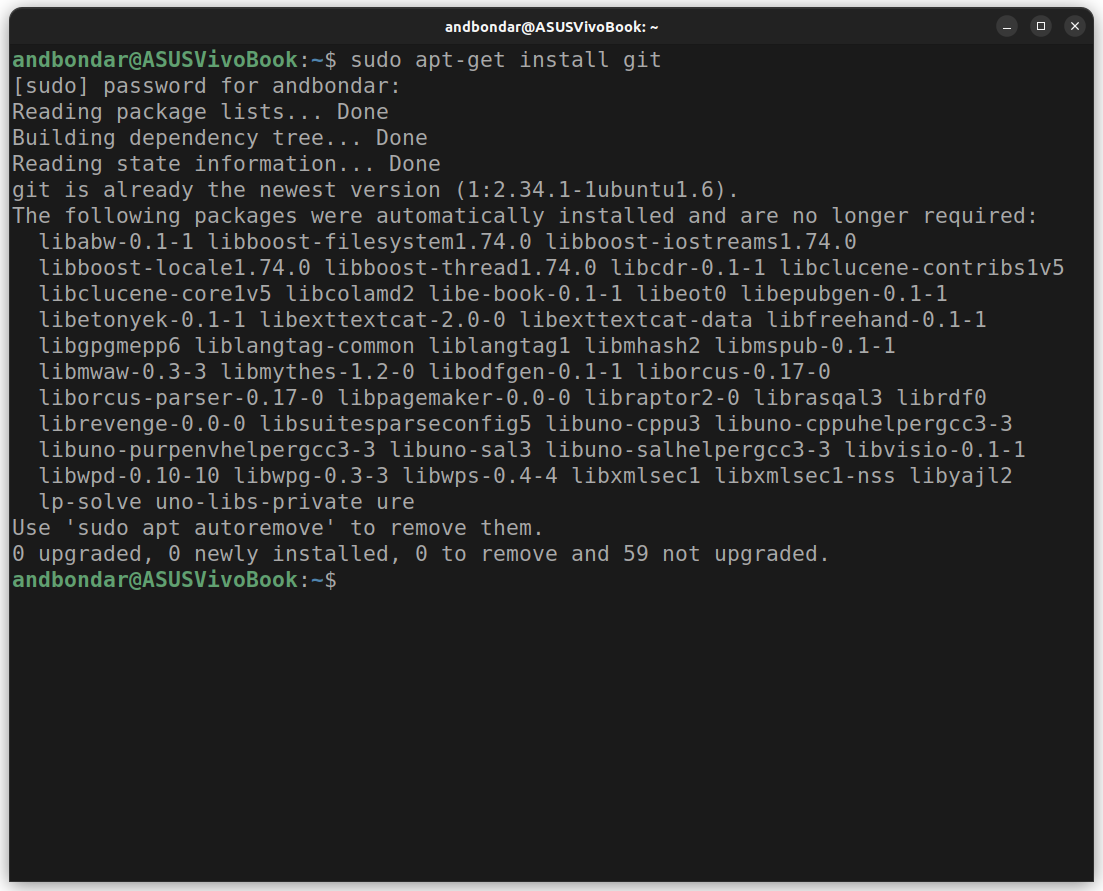
\includegraphics[width=0.7\textwidth]{Screenshot from 2023-02-14 10-47-05.png}
	\caption{Установка git}
	\label{fig:git:install}
\end{figure}

\subsection{Настройка git}
\begin{enumerate}
	\item Открываем терминал.
	\item Необходимо выполнить следующие команды:
	\begin{verbatim}
		git config --global user.name "Your Name"
		git config --global user.email "your_email@whatever.com"
	\end{verbatim}
	\item Необходимо выполнить следующие команды:
	\begin{verbatim}
		git config --global core.autocrlf input
		git config --global core.safecrlf warn
	\end{verbatim}
	\item Необходимо выполнить следующую команды:
	\begin{verbatim}
		git config --global core.quotepath off
	\end{verbatim}
	\item Необходимо выполнить следующую команды:
	\begin{verbatim}
		git config --global core.quotepath off
	\end{verbatim}
\end{enumerate}
Для проверки верности всех введенных команд, введите:
\begin{verbatim}
	git config --list
\end{verbatim}
\begin{figure}[h!tp]
	\centering
	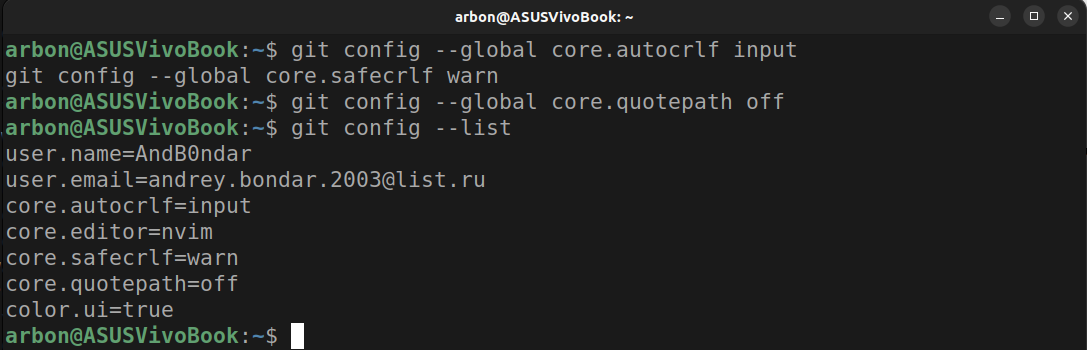
\includegraphics[width=0.8\textwidth]{Screenshot from 2023-02-14 11-05-52.png}
	\caption{Настройка git}
	\label{fig:git:config}
\end{figure}

\section{Создарние локальный репозиторий и добавление в него несколько файлов}

Выполняем команду \texttt{git init}.
После выполнения данной команды, должно высветиться данное сообщение, показанное на рис. \ref{fig:git:init}.
\begin{figure}[h!tp]
	\centering
	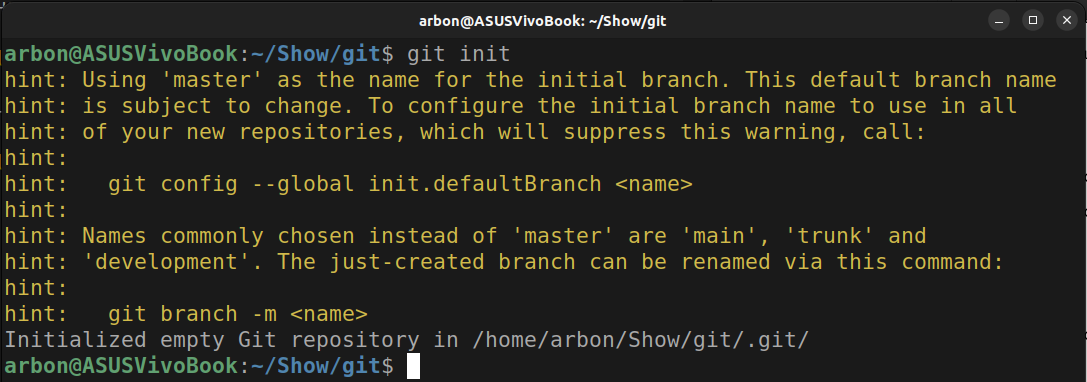
\includegraphics[width=0.8\textwidth]{Screenshot from 2023-02-14 11-21-16.png}
	\caption{Создание репозитория git}
	\label{fig:git:init}
\end{figure}

\section{Добавление файлов в репозиторий}
Далее, командой \texttt{touch file} создадим несколько текстовый файлов.
Чтобы добавить файл в репозиторий необходимо выполнить следующее:
\begin{enumerate}
	\item Вводим команды:
	\begin{verbatim}
		git add <Название вашего файла>
		git commit -m "Ваш текст для коммита"
	\end{verbatim}
\item Чтобы проверить состояние репозитория,
	выполним команду: \texttt{git~status}.
	Команда проверки состояния сообщит, что коммитить нечего.
	Это означает, что в репозитории хранится текущее состояние
	рабочего каталога, и нет никаких изменений, ожидающих записи.
\end{enumerate}
Результат этих действий показан на рисунке \ref{fig:git:first_commit}.
\begin{figure}[h!tp]
	\centering
	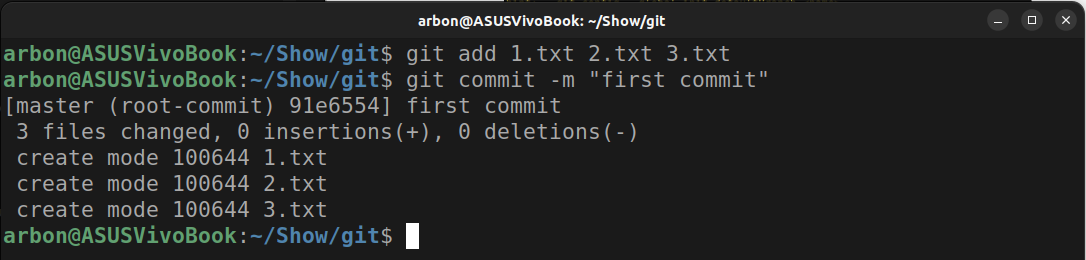
\includegraphics[width=0.8\textwidth]{Screenshot from 2023-02-14 11-32-30.png}
	\caption{Добавление файлов в репозиторий и первый коммит}
	\label{fig:git:first_commit}
\end{figure}

\section{Изменение файла}

Далее внесем изменения в один из файлов. Путем перенаправления вывода команды
\texttt{echo} в файл. Добавим изменения в индекс командой:
\texttt{git~add~<имя~файла>}. Чтобы проверить внесение команды в индекс,
git предоставляет команду \texttt{git~status}. Все эти действия отображены
на рисунке \ref{fig:git:changes}.

\begin{figure}[h!tp]
	\centering
	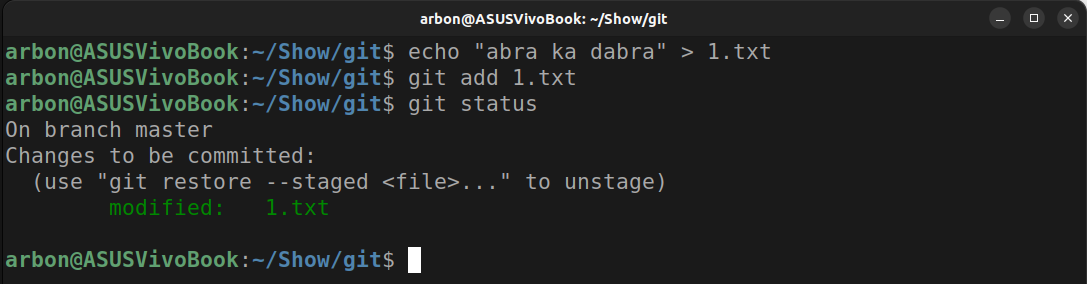
\includegraphics[width=0.8\textwidth]{Screenshot from 2023-02-18 19-43-35.png}
	\caption{Индексирование изменений и их проверка}
	\label{fig:git:changes}
\end{figure}

\section{Коммит}

Теперь, чтобы сохранить изменнения в репозитории, необходимо сделать коммит.
Для этого существует команда \texttt{git~commit~-m~"текст~коммита"}
(см.~рисунок~\ref{fig:git:second_commit}).
Флаг \texttt{-m} позволяет сразу добавить коментарий при вводе команды, без
него git, для комментария, откроет текстовый редактор,
установленный по умолчанию, обычно это vim.

\begin{figure}[h!tp]
	\centering
	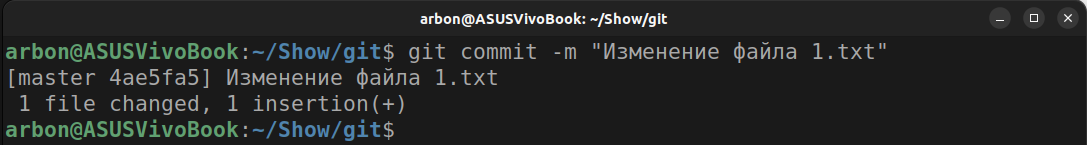
\includegraphics[width=0.8\textwidth]{Screenshot from 2023-02-18 19-51-38.png}
	\caption{Коммит}
	\label{fig:git:second_commit}
\end{figure}

\section{Как работает индексация}
Выполним подряд следующие шаги:
\begin{enumerate}
	\item Изменим еще один файл.
	\item Добавим это изменение в индекс git.
	\item Изменим файл еще раз.
	\item Проверим состояние и произведем коммит проиндексированного
		изменения.
	\item Добавим второе изменение в индекс,
		а затем проверим состояние с помощью команды \texttt{git~status}.
	\item Сделаем коммит второго изменения.
\end{enumerate}

Результаты проделанных шагов проиллуюстрированны на
рисунках~\ref{fig:git:first_indexed_change}-\ref{fig:git:second_indexed_change}.

\begin{figure}[h!tp]
	\centering
	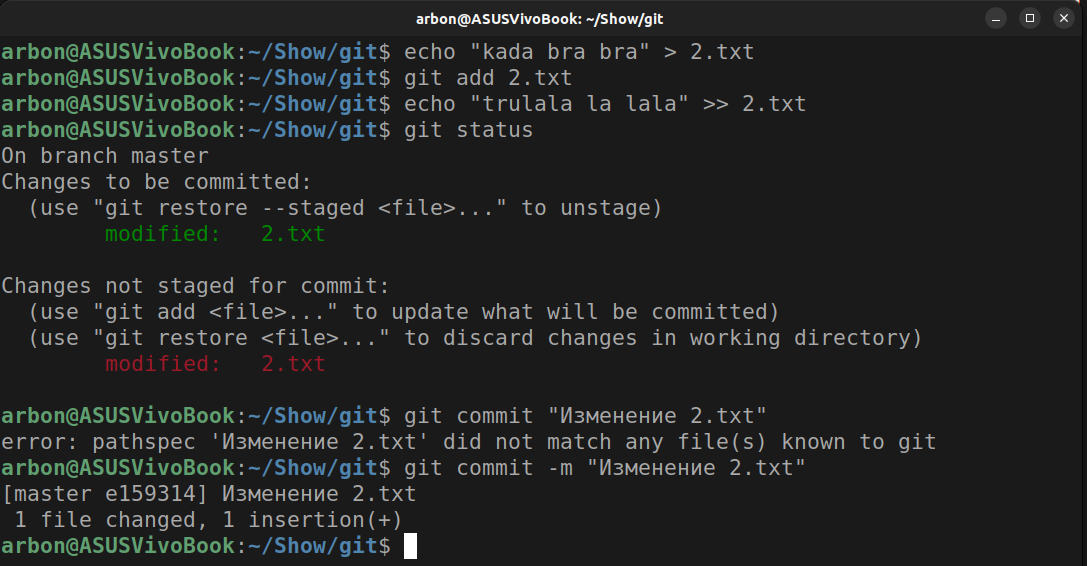
\includegraphics[width=0.7\textwidth]{Screenshot from 2023-02-18 20-09-49.png}
	\caption{Коммит первого проиндексированного изменения}
	\label{fig:git:first_indexed_change}
\end{figure}

\begin{figure}[h!tp]
	\centering
	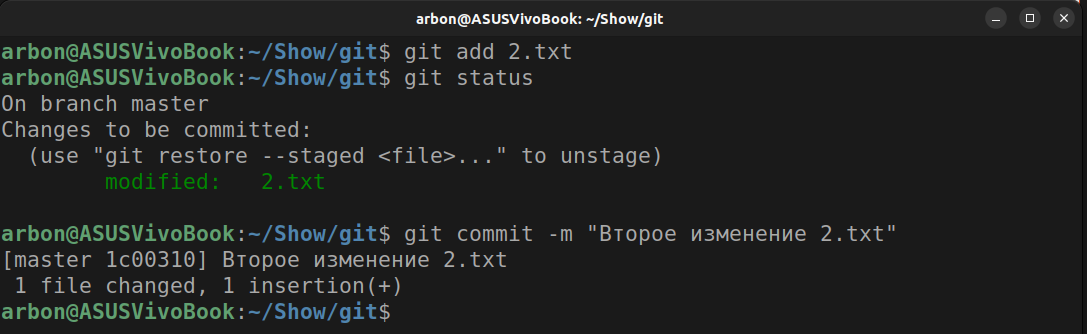
\includegraphics[width=0.7\textwidth]{Screenshot from 2023-02-18 20-14-31.png}
	\caption{Коммит второго проиндексированного изменения}
	\label{fig:git:second_indexed_change}
\end{figure}

\section{История коммитов}
Для просмотра истории коммитов используется команда: \texttt{git~log}
(Рисунок \ref{fig:git:log}).

\begin{figure}[h!tp]
	\centering
	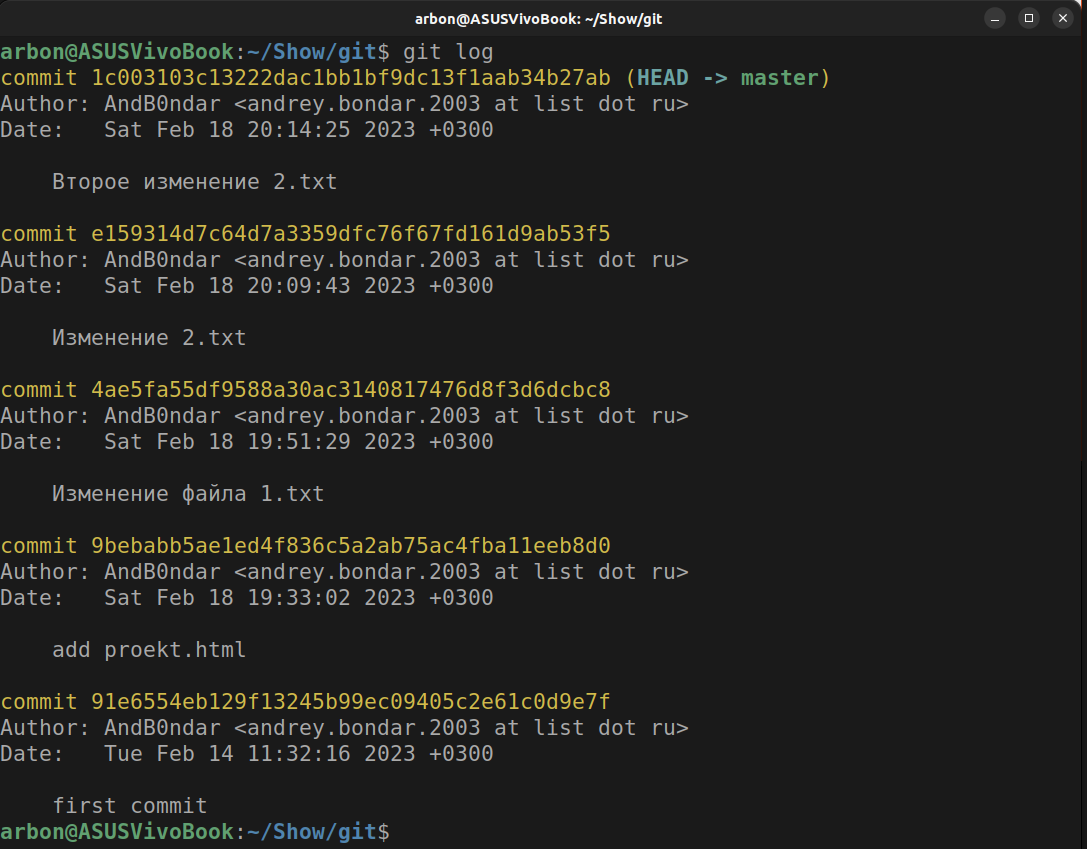
\includegraphics[width=0.8\textwidth]{Screenshot from 2023-02-18 20-21-34.png}
	\caption{История коммитов}
	\label{fig:git:log}
\end{figure}

Для уточнения формата лога используется флаг \verb|--pretty=format:”...”|.

Для примера выполните команду:
\begin{verbatim}
git log --pretty=format:"%h %ad | %s%d [%an]" --graph --date=short
\end{verbatim}

Рассмотрим её в деталях:
\begin{itemize}
	\item \texttt{\%h} — укороченный хэш коммита
	\item \texttt{\%d} — дополнения коммита («головы» веток или теги)
	\item \texttt{\%ad} — дата коммита
	\item \texttt{\%s} — комментарий
	\item \texttt{\%an} — имя автора
	\item \verb|--graph| — отображает дерево коммитов в виде ASCII-графика
	\item \verb|--date=short| — сохраняет формат даты коротким
\end{itemize}

Приведем пирмер одного из форматирования вывода
истории~(см.~рис.~\ref{fig:git:flog}).

\begin{figure}[h!tp]
	\centering
	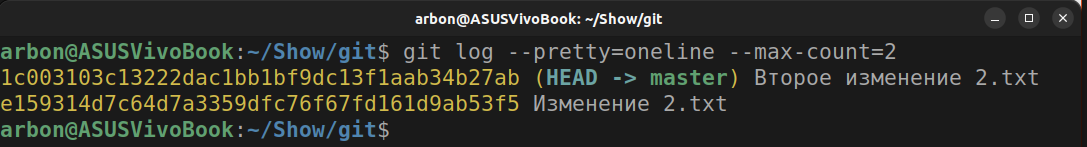
\includegraphics[width=0.8\textwidth]{Screenshot from 2023-02-18 20-35-49.png}
	\caption{Форматирование истории коммитов}
	\label{fig:git:flog}
\end{figure}

\section{Отмена изменений}
Для отмены изменений в репозитории существует команда \texttt{git~reset},
которая переместит HEAD и текущую ветку обратно туда, куда вы укажете,
отказавшись от любых коммитов, которые могут быть оставлены позади.
Далее останется очистить индекс командой \texttt{git restore}.
И так, чтобы вернуть директорию в предыдущее состояние введем
слудующие команды:
\begin{verbatim}
	git reser --soft HEAD^
	git restore --staged 2.txt
\end{verbatim}
Результат этих команд проиллуюстрирован на рисунке \ref{fig:git:reset}.

\begin{figure}[h!tp]
	\centering
	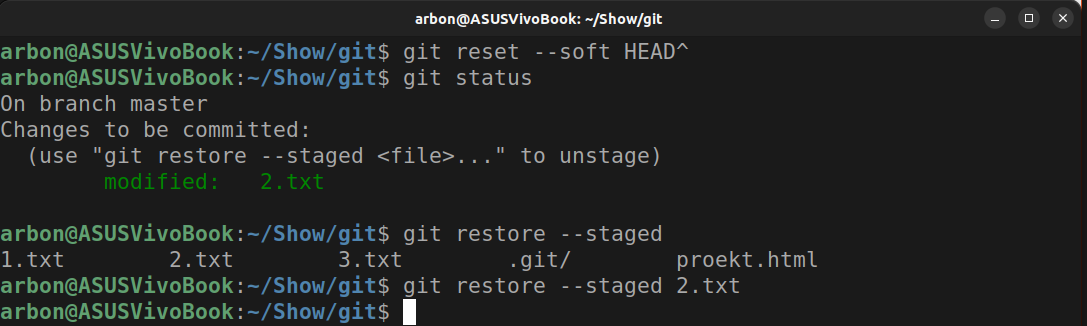
\includegraphics[width=0.8\textwidth]{Screenshot from 2023-02-18 20-54-01.png}
	\caption{Возвращение рабочего каталога к предыдущему состоянию}
	\label{fig:git:reset}
\end{figure}

\section{Создание тега}

Git использует два основных типа тегов: легковесные и аннотированные.

Легковесный тег ---это что-то очень похожее на ветку,
которая не изменяется --- просто указатель на определённый коммит.

А вот аннотированные теги хранятся в базе данных Git как полноценные объекты.
Они имеют контрольную сумму, содержат имя автора, его e-mail и дату создания,
имеют комментарий и могут быть подписаны и проверены с помощью
GNU Privacy Guard (GPG). Обычно рекомендуется создавать аннотированные теги,
чтобы иметь всю перечисленную информацию; но если вы хотите сделать
временную метку или по какой-то причине не хотите сохранять остальную
информацию, то для этого годятся и легковесные.

\subsection{Аннотированные теги}
Создание аннотированного тега в Git выполняется легко.
Самый простой способ --- это указать -a при выполнении команды tag:

\begin{verbatim}
	git tag -a <имя тега> -m "my version 1.4"
\end{verbatim}

Опция -m задаёт сообщение, которое будет храниться вместе с тегом.
Если не указать сообщение, то Git запустит редактор,
чтобы вы смогли его ввести.

\subsection{Легковесный теги}
Легковесный тег --- это ещё один способ пометить коммит. По сути,
это контрольная сумма коммита, сохранённая в файл --- больше никакой
информации не хранится. Для создания легковесного тега не передавайте
опций -a, -s и -m, укажите только название:

\begin{verbatim}
	git tag <имя тега>
\end{verbatim}

Создание легковесного тега показано на рисунке \ref{fig:git:tag}.

\begin{figure}[h!tp]
	\centering
	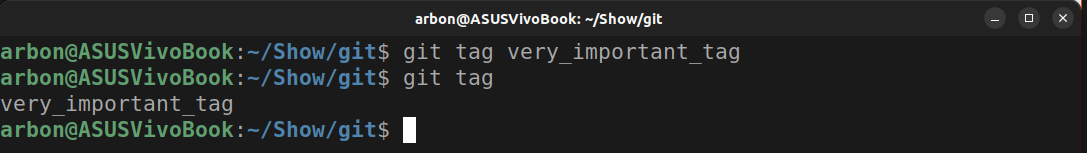
\includegraphics[width=0.9\textwidth]{Screenshot from 2023-02-18 21-08-19.png}
	\caption{Создание тега}
	\label{fig:git:tag}
\end{figure}

\section{Отмена изменений в индексе}
\subsection{Отмена изменений (до индексации)}
Для отмены изменений необходимо выполнить команду:
\begin{verbatim}
	git checkout master
\end{verbatim}
Результат выполнения этой команды показан
на рисунке~\ref{fig:git:checkout:b_indx}.
\begin{figure}[h!tp]
	\centering
	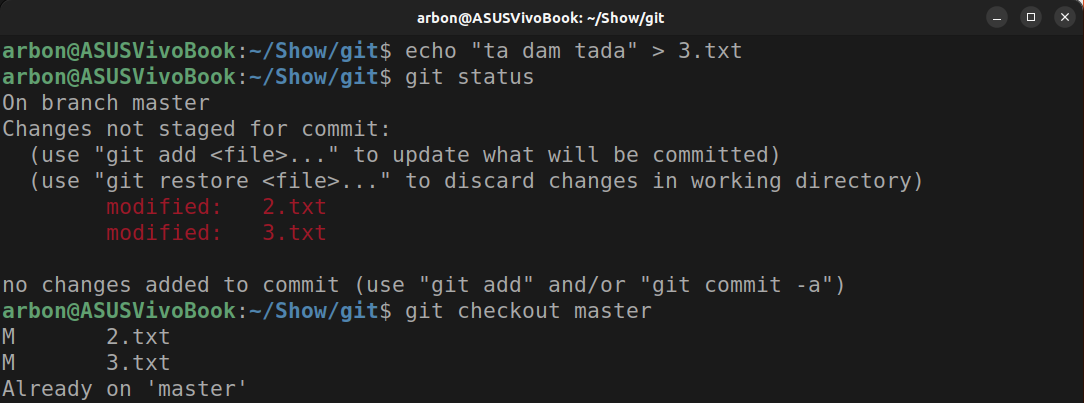
\includegraphics[width=0.7\textwidth]{Screenshot from 2023-02-19 15-24-48.png}
	\caption{Отмена изменений (до индексации)}
	\label{fig:git:checkout:b_indx}
\end{figure}

\subsection{Отмена изменений (после индексации)}
Для отмены изменений, уже проиндексированных, необходимо выполнить команду:
\begin{verbatim}
	git reset HEAD имя_файла
\end{verbatim}
Результат выполнения этой команды показан на рисунке~\ref{fig:git:restore}.
\begin{figure}[h!tp]
	\centering
	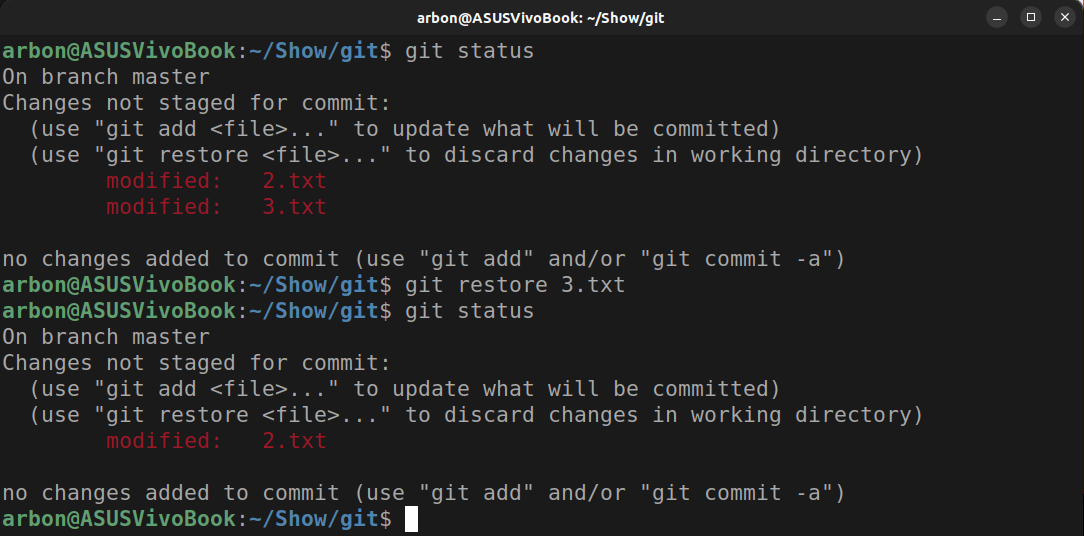
\includegraphics[width=0.8\textwidth]{Screenshot from 2023-02-19 15-27-04.png}
	\caption{Отмена изменений (после индексации)}
	\label{fig:git:restore}
\end{figure}

\section{Отмена коммита}
Для отмены изменений в репозитории существует команда: \texttt{git~reset},
которая переместит HEAD и текущую ветку обратно туда, куда вы укажете,
отказавшись от любых коммитов, которые могут быть оставлены позади.
Данное действие уже показано на рисунке \ref{fig:git:reset}.
